\documentclass[11pt]{article}
%\usepackage[latin1]{inputenc}
\usepackage[french]{babel}
\usepackage{graphicx}

\usepackage{amsmath}
\usepackage{amssymb}

\usepackage{times}

%%%%%%%%%%%%%%%%%%%%%%%%%%%%%%%%%%%%%%%%%%%%%%
\usepackage{color}

\def\textRed{\color{red}}
\def\textBlack{\color{black}}
\def\textBlue{\color{blue}}
\def\Blue#1{{\color{blue}{#1}}}
\def\Red#1{{\color{red}{#1}}}
\def\Green#1{{\color{green}{#1}}}
%\def\ Magenta#1{{\color{magenta}{#1}}}
\usepackage{FFF}
%%%%%%%%%%%%%%%%%%%%%%%%%%%%%%%%%%%%%%%%%%%%%%%%%

\oddsidemargin -0.2cm \textwidth 16.8cm \topmargin -2.8cm
\headheight 0.0cm \textheight 26.80cm
\parindent 0pt
\parskip 8pt

\newcommand{\R}{\ensuremath{\mathbb R}}
\newcommand{\N}{\ensuremath{\mathbb N}}
\newcommand{\Z}{\ensuremath{\mathbb Z}}
\newcommand{\C}{\ensuremath{\mathbb C}}
\def\Rtwo{\R^2}
\def\ds{\displaystyle}
\newcommand{\uim}{{\bf i}}
\def\Th{\mathcal{T}_{h}}
\def\Som{\mathcal{S}_{\Th}}
\def\SomO{\mathcal{S}^{\circ}_{\mathcal{T}_{h}}}
\def\SomG{\mathcal{S}^{\Gamma}_{\mathcal{T}_{h}}}

%\pagestyle{empty}

\begin{document}
\noindent
{\rule{\textwidth}{.2mm}}\\
Universit{\'e} Pierre et Marie Curie  -- Paris 6
\hfill
Projet 2\\
Informatique scientifique en C++\hfill
Mars 2005\\
{\rule{\textwidth}{.2mm}}\\[2mm]

\vspace{-1cm}
\begin{center}
\framebox{\Large\sl
\begin{minipage}{14cm}
  \begin{center}
  Projet 2 - premi{\`e}re partie\\
Utilisation de \texttt{FreeFem++} et des classes \texttt{sfem}
pour la m{\'e}thode des {\'e}l{\'e}ments finis $P^1$
\end{center}
\end{minipage}}
\end{center}


\framebox{\centerline{\bf Q1 : Construction d'une triangulation
avec FreeFem++}}
%%%%%%%%%%%%%%%%%%%%%%%%%%%%%%%%%%%%%%%%%%%%%%%%%

\begin{enumerate}
\item   Le script {\em cercle.edp} contient des instructions qui
permettent au logiciel \texttt{FreeFem++}  de g{\'e}n{\'e}rer le maillage
d'un cercle, avec $n$ points de discr{\'e}tisation distribu{\'e}s sur la
fronti{\`e}re. Tester le script\footnote{Pour t{\'e}l{\'e}charger et installer
\texttt{FreeFem++} sur votre machine (sous Windows ou Linux),
consulter la page www.freefem.org.}  pour diff{\'e}rents $n$.

Analyser la structure du fichier {\em cercle.msh} qui contient la
triangulation g{\'e}n{\'e}r{\'e}e avec ce script.




\begin{figure}[h]
  \begin{center}  
  \includegraphics[width=0.8\textwidth]{cercle10.pdf}
    \caption{Utilisation de freefem++ pour construire le maillage d'un cercle pour lequel le nomrbre n de points du maillage situ�s sur la fronti�re est 10. }
    \label{fig:1}
  \end{center}
\end{figure}
\medskip




\begin{figure}[h]
  \begin{center}  
  \includegraphics[width=0.8\textwidth]{cercle100.pdf}
    \caption{idem avec n=100 }
    \label{fig:2}
  \end{center}
\end{figure}
\medskip



\item Suivant le mod{\`e}le pr{\'e}c{\'e}dent, {\'e}crire un script FreeFem++ pour
g{\'e}n{\'e}rer le maillage du rectangle $[0,L_1]\times[0,L_2]$, en
optimisant la forme des triangles du maillage (le rapport $L/n$
doit {\^e}tre le m{\^e}me pour chaque morceau de fronti{\`e}re de longueur $L$
sur lequel on distribue $n$ points de discr{\'e}tisation).




\begin{figure}[h]
  \begin{center}  
  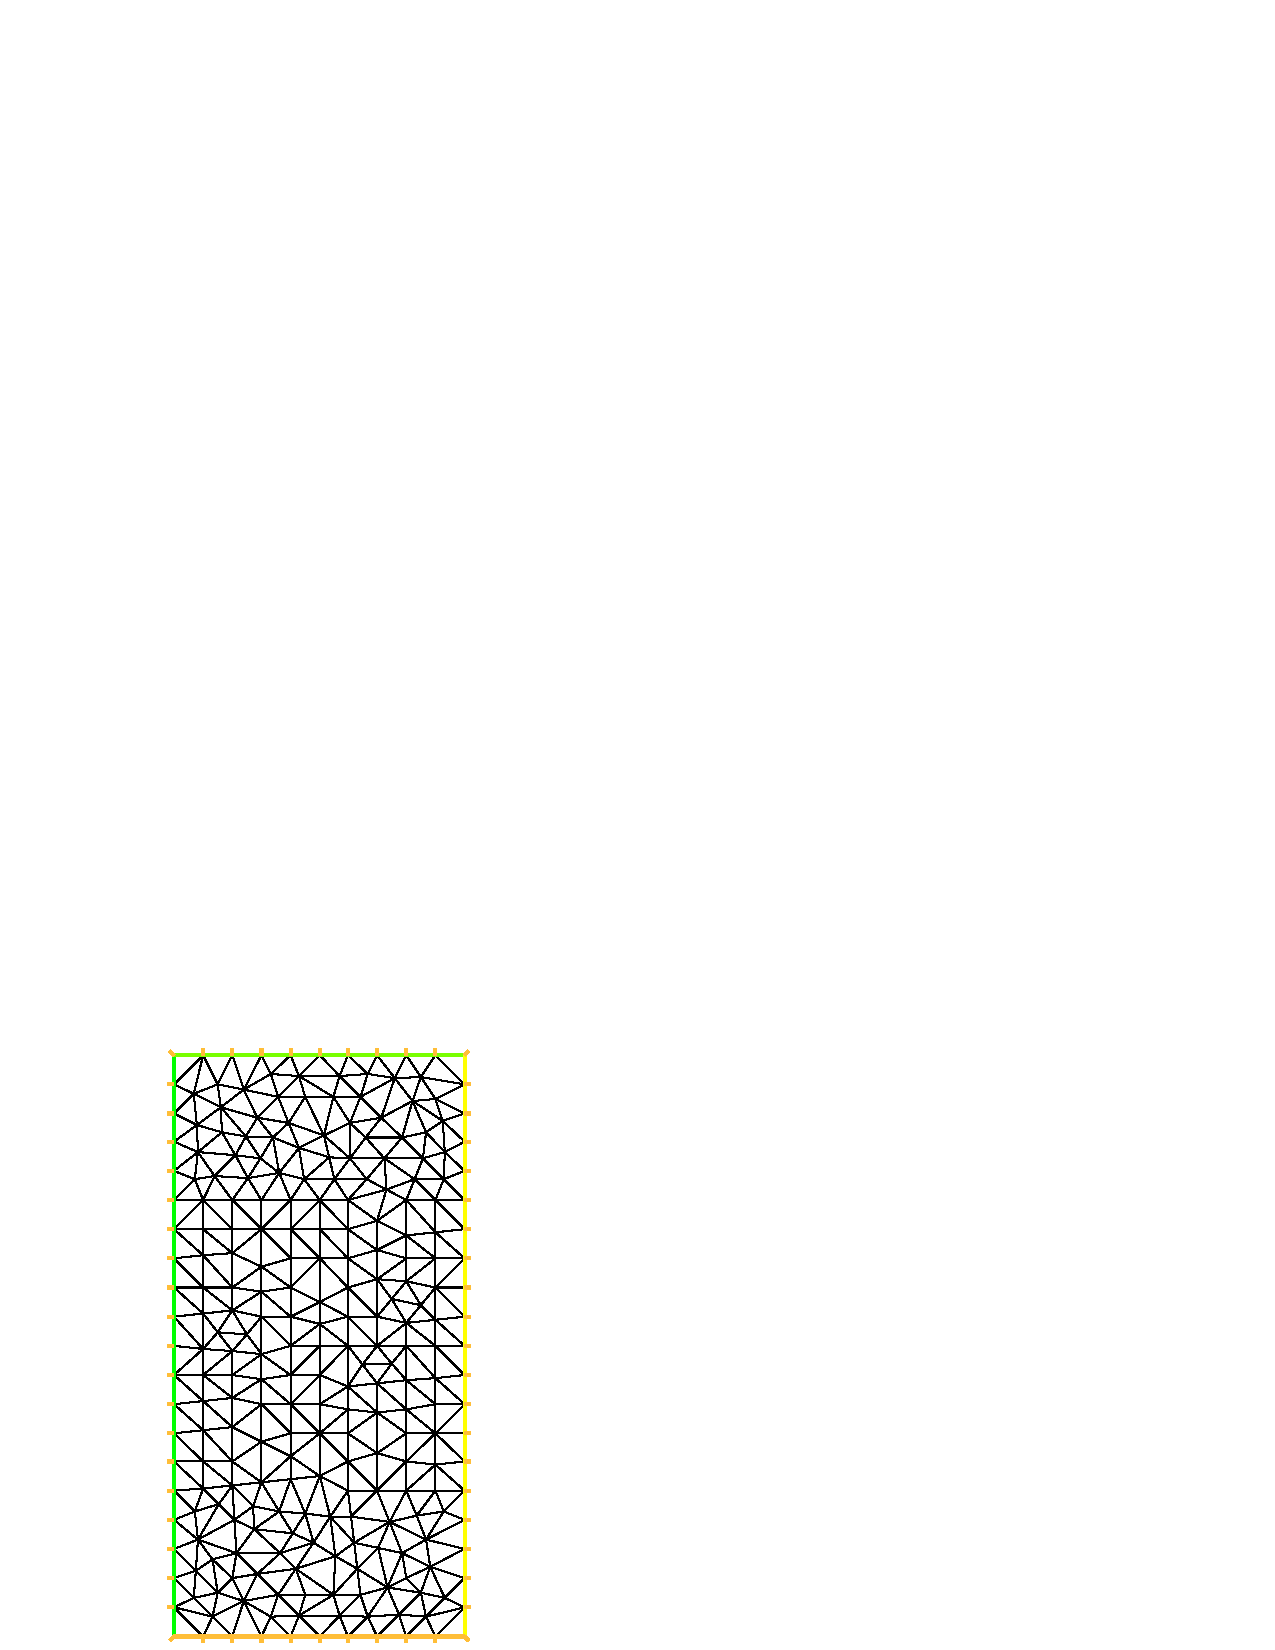
\includegraphics[width=0.8\textwidth]{rectangle.pdf}
    \caption{maillage uniforme d'un rectangle dont la largeur vaut 1 et la longueur vaut 2   }
    \label{fig:3}
  \end{center}
\end{figure}
\medskip


\item  Construire une triangulation avec \texttt{FreeFem++} d'un
carr{\'e} unit{\'e} avec un trou elliptique (les trous sont obtenus en
changeant le sens de parcours de la fronti{\`e}re).



\begin{figure}[h]
  \begin{center}  
  \includegraphics[width=0.8\textwidth]{carretroue.pdf}
    \caption{maillage d'un carre poss{\'e}dant un trou elliptique }
    \label{fig:4}
  \end{center}
\end{figure}
\medskip


\item  Changer le sens de parcours de l'ellipse et l'utiliser pour
contr{\^o}ler le raffinement du maillage dans cette r{\'e}gion.



\begin{figure}[h]
  \begin{center}  
  \includegraphics[width=0.8\textwidth]{carretroueraf.pdf}
    \caption{maillage d'un carre poss{\'e}dant un trou elliptique � l'int{\'e}rieur
 duquel le maillage a {\'e}t{\'e} raffin{\'e}}
    \label{fig:5}
  \end{center}
\end{figure}
\medskip


\end{enumerate}

\framebox{\centerline{\bf Q2 : R{\'e}solution d'une EDP avec
FreeFem++}}
%%%%%%%%%%%%%%%%%%%%%%%%%%%%%%%%%%%%%%%%%%%%%%%%%

Le script {\em cercle\_lap.edp} r{\'e}sout l'EDP suivante
\begin{equation}
  -\Delta u = f \quad \mbox{sur} \quad \Omega, \quad
\mbox{et}\quad u|_{\Gamma}= g , \label{eq-edp1}
\end{equation}
avec le choix particulier :
\begin{equation}
  g(x,y)= x^2+2 y^2, \qquad  f(x,y)= -6,
 \label{eq-edp1bc}
\end{equation}
et le domaine $\Omega$ le cercle de rayon $R$, centr{\'e} en origine.

\begin{enumerate}
  \item Tester le script et analyser la syntaxe utilis{\'e}e pour
r{\'e}soudre la formulation variationnelle. Rajouter dans le script la
visualisation de la solution exacte pour ce probl{\`e}me.




\begin{figure}[h]
  \begin{center}  
  \includegraphics[width=0.8\textwidth]{xsplot.pdf}
    \caption{ solution de l'equation
      $  -\Delta u = f $ et $u|_{\Gamma}= g$ 
      avec le choix particulier :
      $ g(x,y)= x^2+2 y^2$, $\qquad$  $f(x,y)= -6$ 
    }
    \label{fig:6}
  \end{center}
\end{figure}
\medskip


\begin{figure}[h]
  \begin{center}  
  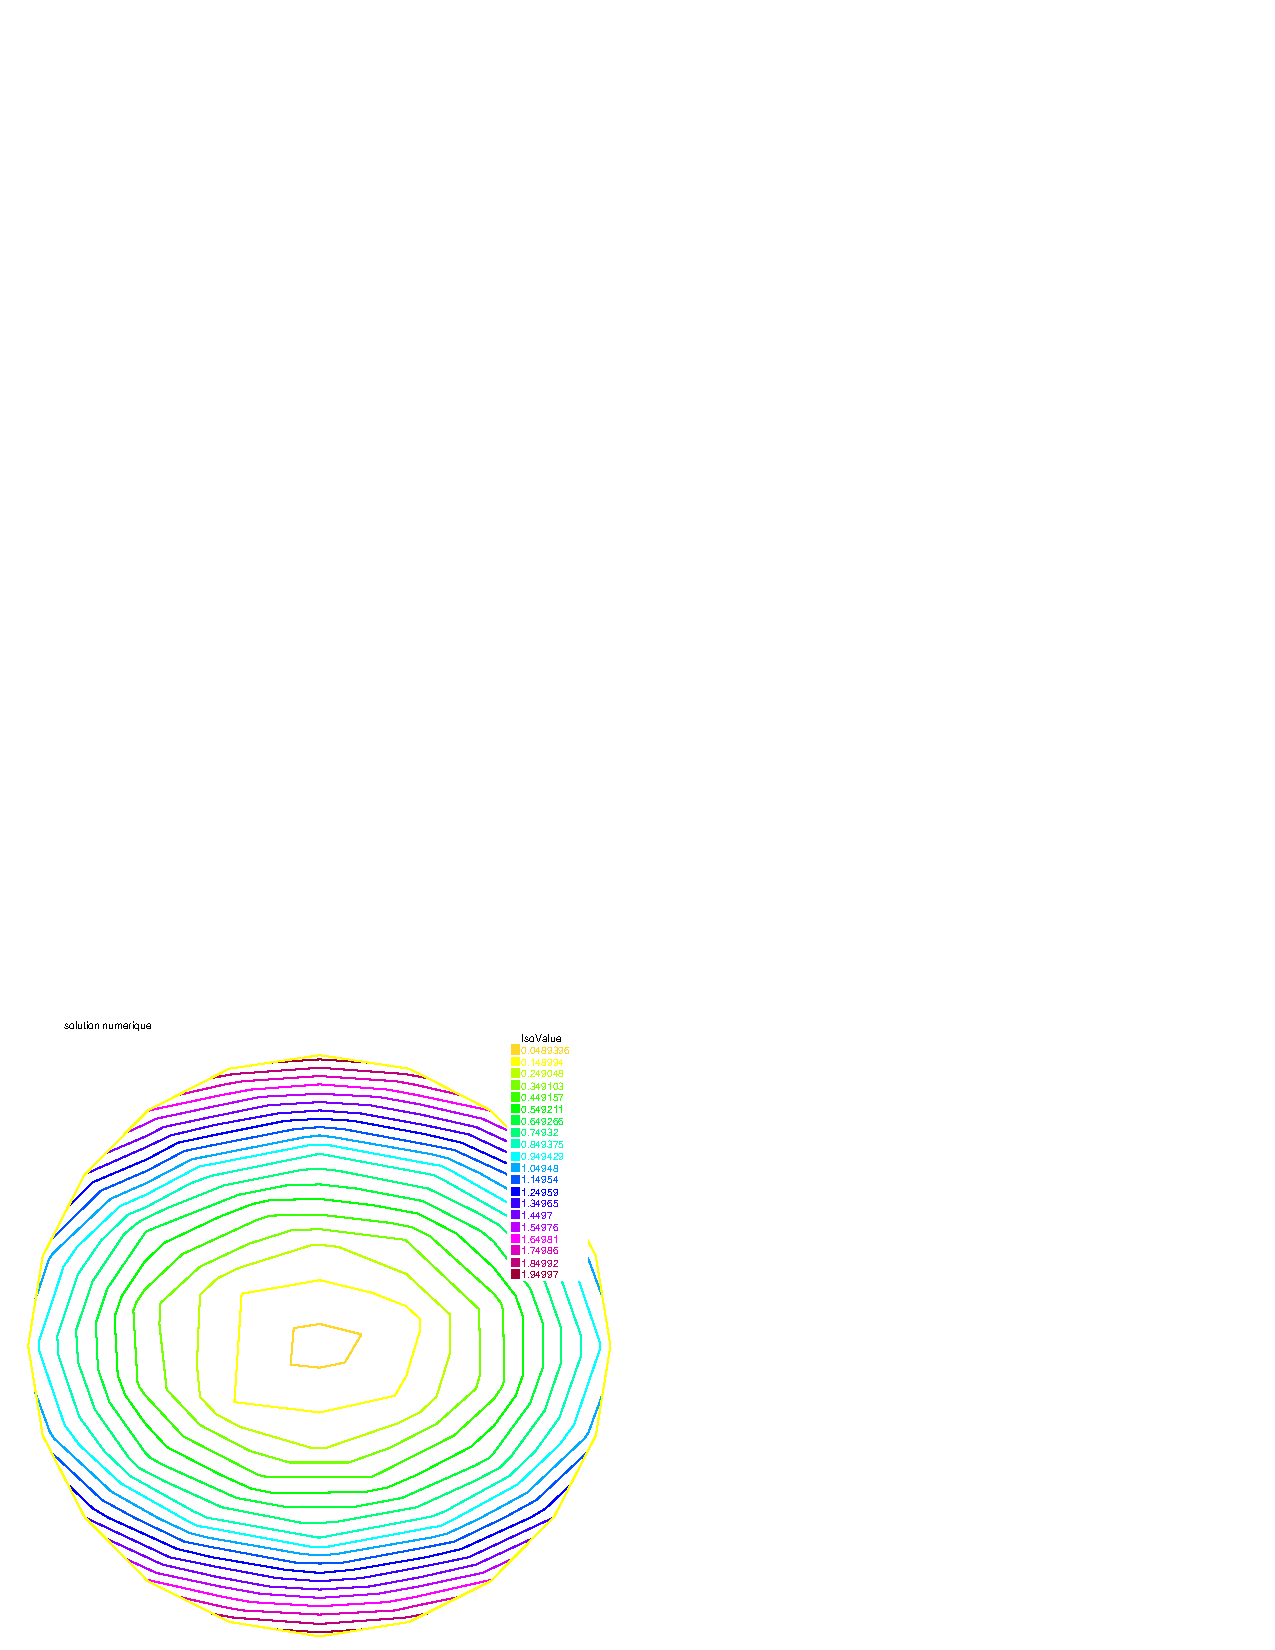
\includegraphics[width=0.8\textwidth]{Q21.pdf}
    \caption{ solution numerique de l'equation
      $  -\Delta u = f $ et $u|_{\Gamma}= g$ 
      avec le choix particulier :
      $ g(x,y)= x^2+2 y^2$, $\qquad$  $f(x,y)= -6$ 
      affichage des isolignes    
    }
    \label{fig:7}
  \end{center}
\end{figure}
\medskip


\begin{figure}[h]
  \begin{center}  
  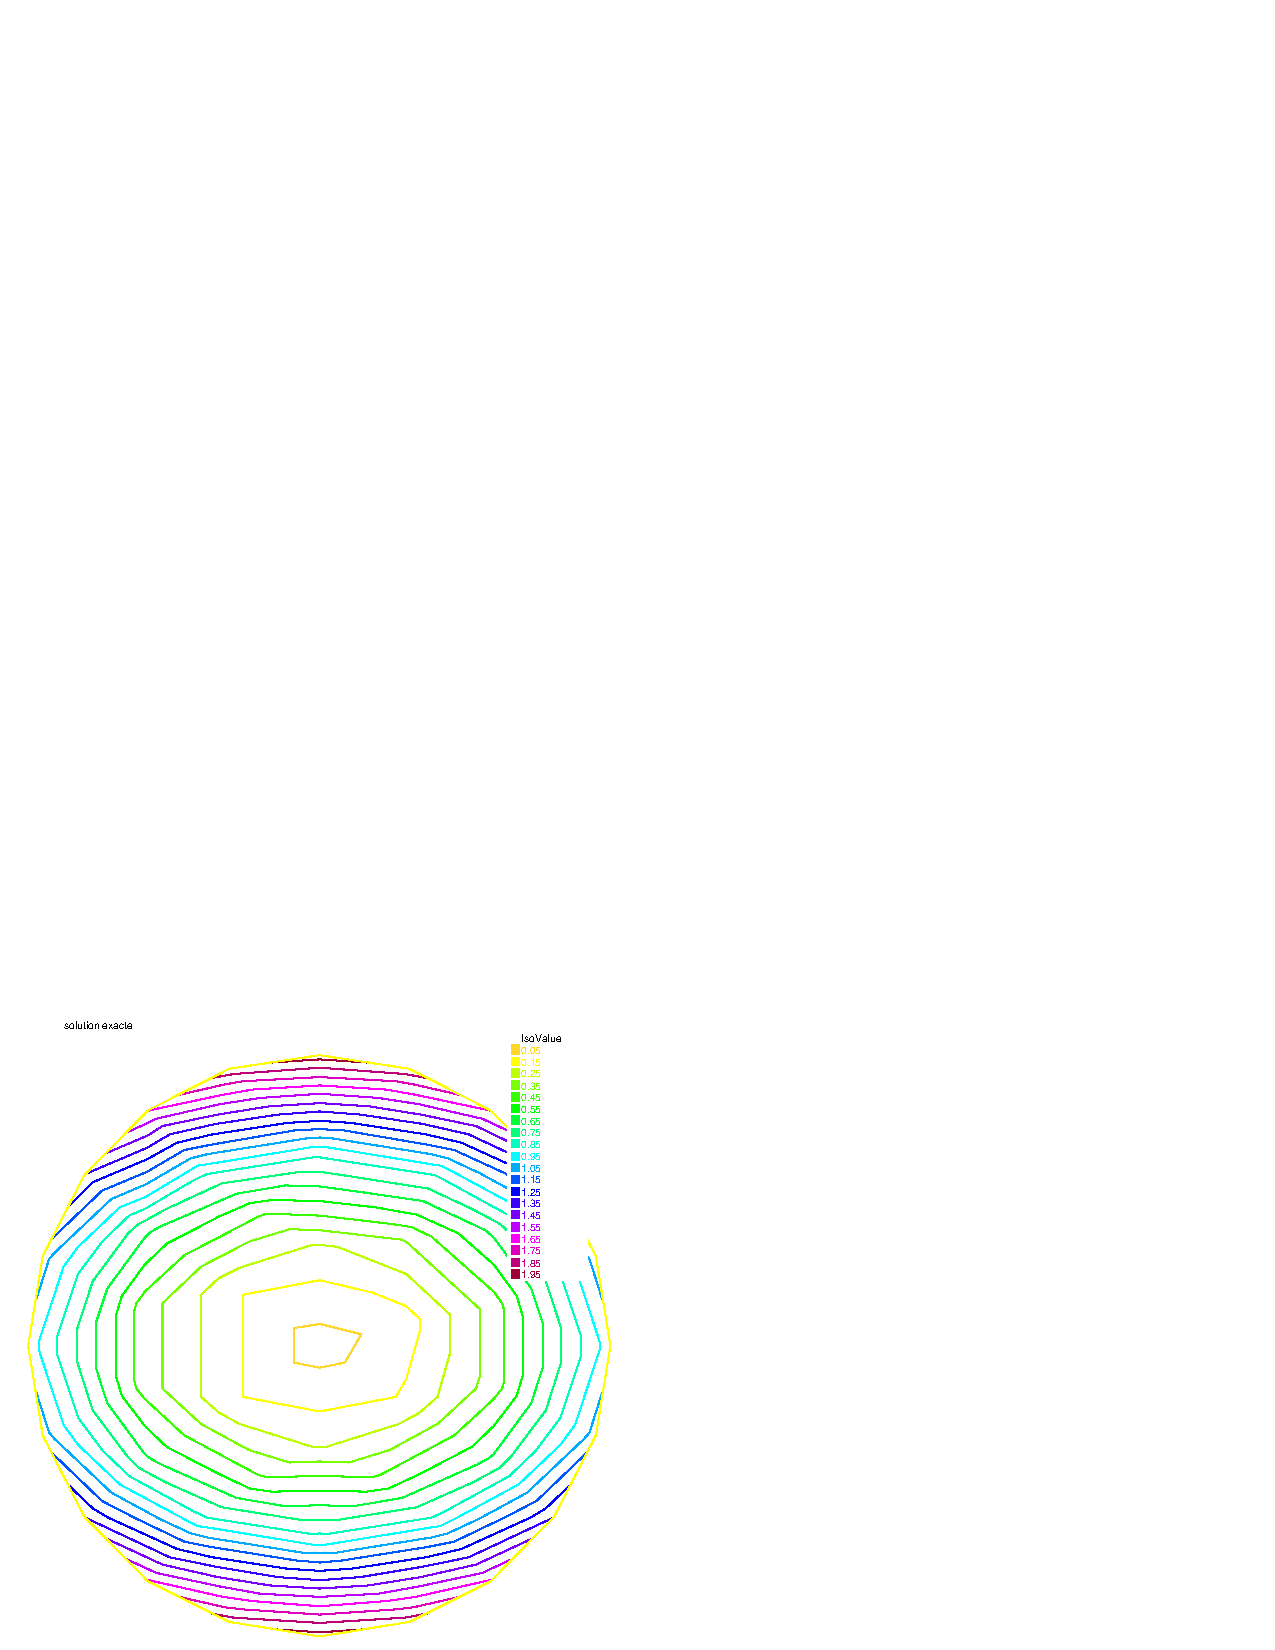
\includegraphics[width=0.8\textwidth]{Q22.pdf}
    \caption{ solution exacte de l'equation
      $  -\Delta u = f $ et $u|_{\Gamma}= g$ 
      avec le choix particulier :
      $ g(x,y)= x^2+2 y^2$, $\qquad$  $f(x,y)= -6$ 
      affichage des isolignes    
    }
    \label{fig:8}
  \end{center}
\end{figure}
\medskip



\item Modifier le script pr{\'e}c{\'e}dent  afin de r{\'e}soudre le probl{\`e}me
\begin{equation}
  -\Delta u +u = f \quad \mbox{sur} \quad \Omega, \quad
\mbox{et}\quad u|_{\Gamma}=g. \label{eq-edp2}
\end{equation}
avec $\Omega=[0,L]\times[0,L]$, $\Gamma=\partial \Omega$. Choisir
$f$ et $g$ afin d'avoir la m{\^e}me solution exacte que pr{\'e}c{\'e}demment.
\end{enumerate}



\begin{figure}[h]
  \begin{center}  
  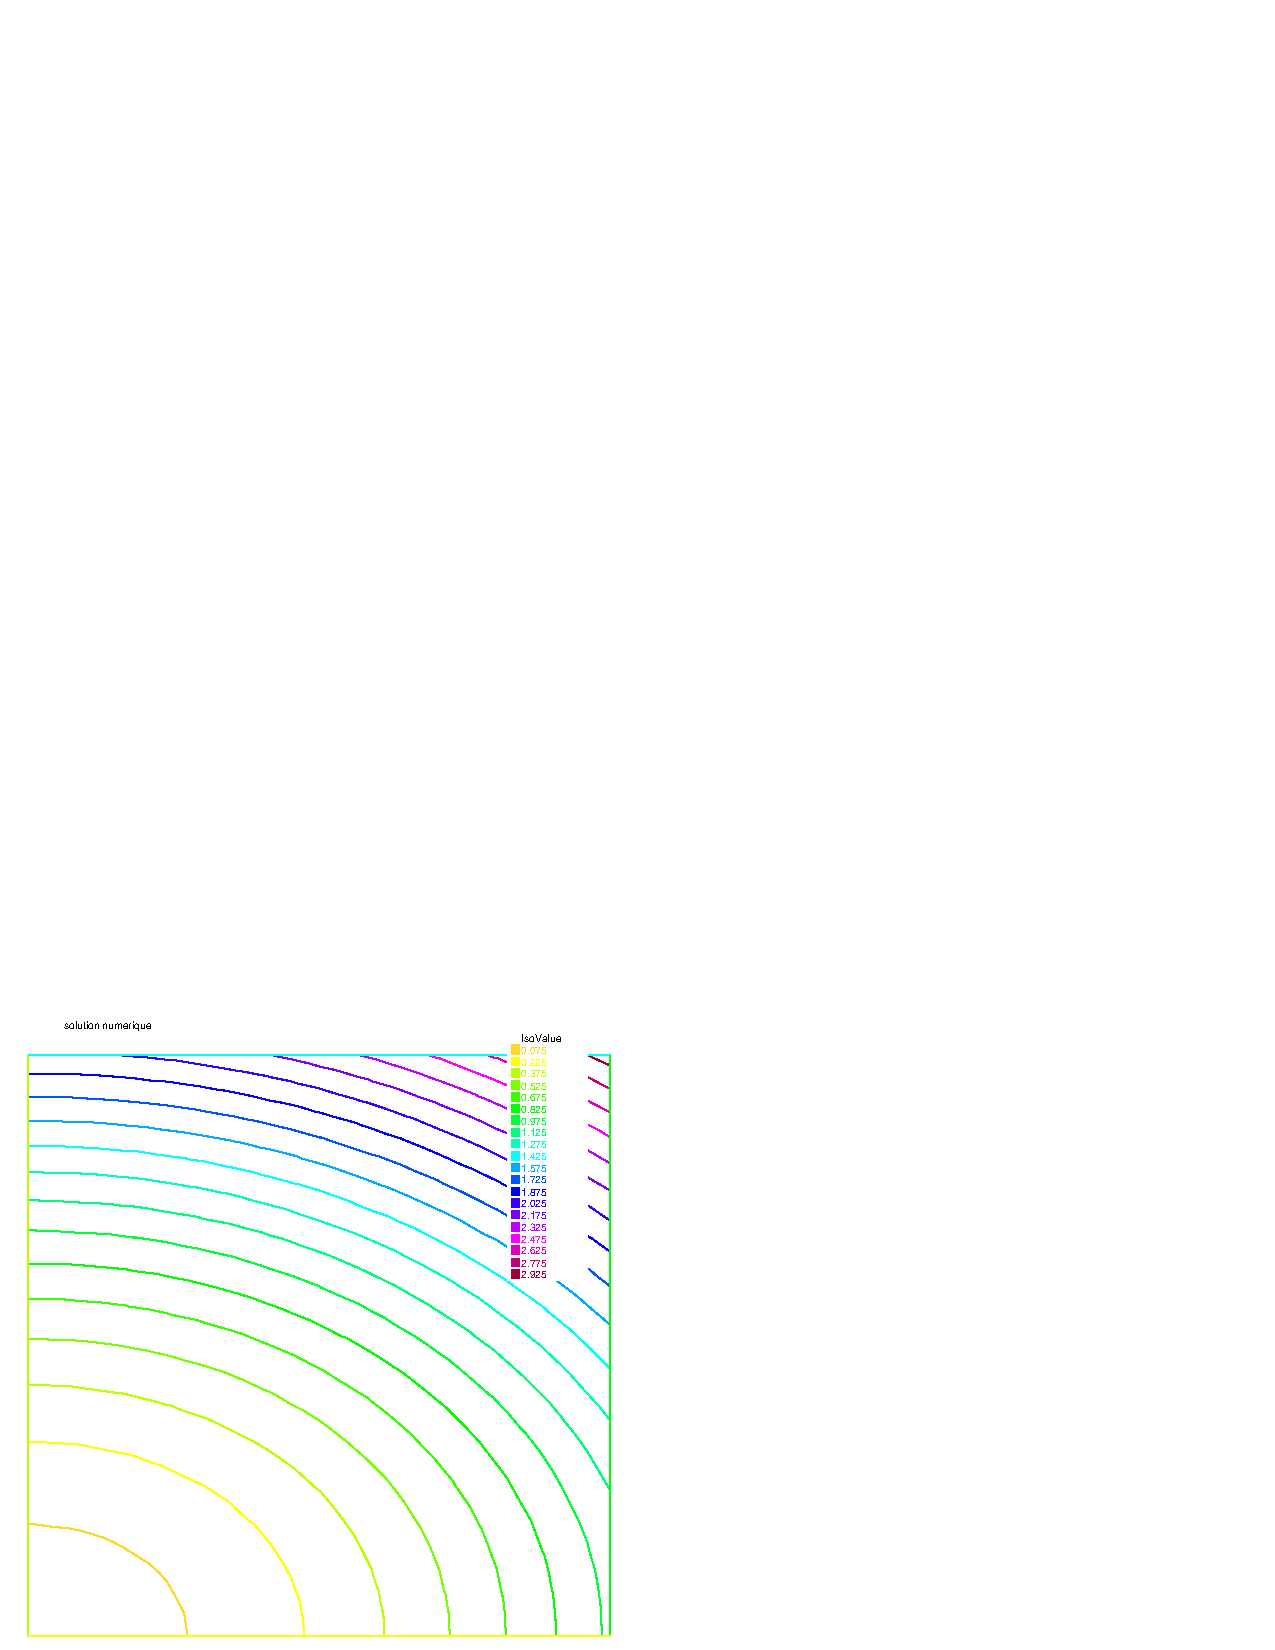
\includegraphics[width=0.8\textwidth]{Q23.pdf}
    \caption{ solution exacte de l'equation
      $  -\Delta u = f $ et $u|_{\Gamma}= g$ 
      avec le choix particulier :
      $ g(x,y)= x^2+2 y^2$, $\qquad$  $f(x,y)= -6$ 
      affichage des isolignes    
    }
    \label{fig:8}
  \end{center}
\end{figure}
\medskip




\begin{figure}[h]
  \begin{center}  
  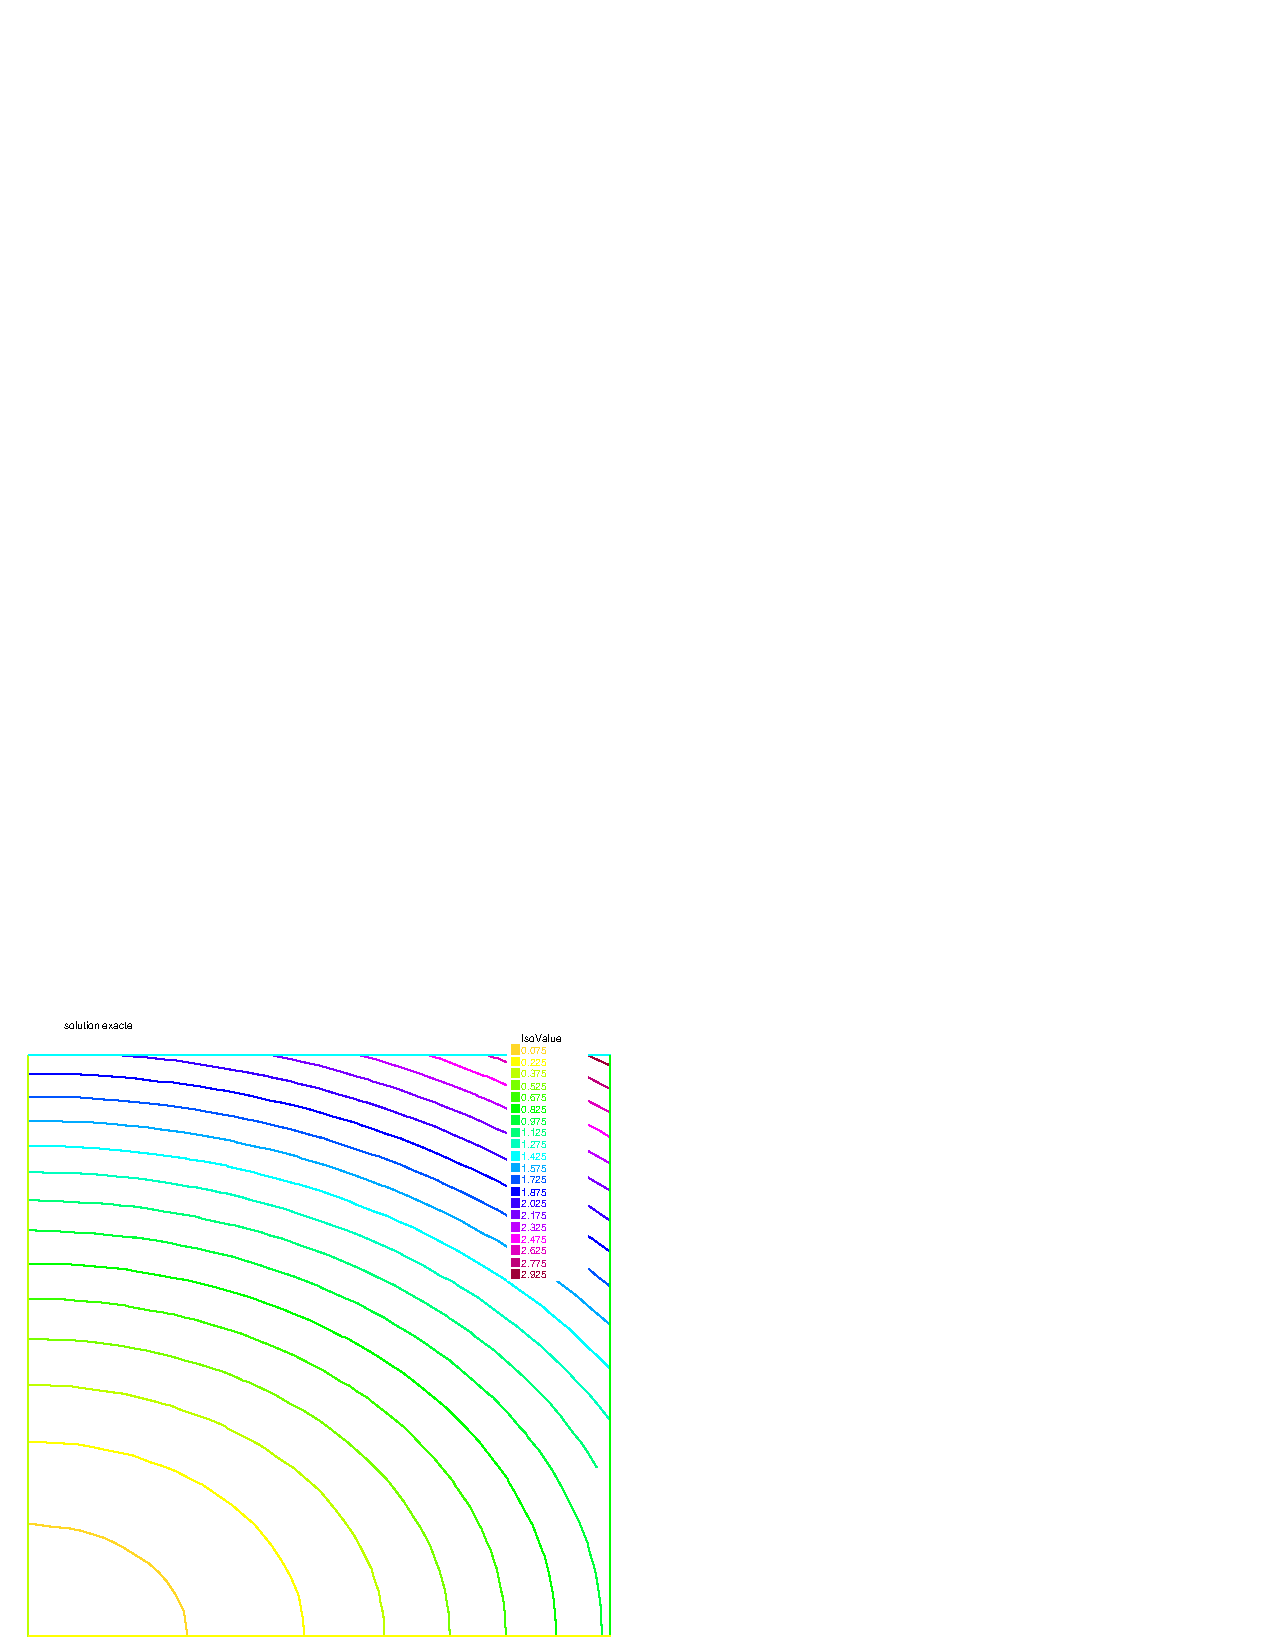
\includegraphics[width=0.8\textwidth]{Q24.pdf}
    \caption{ solution exacte de l'equation
      $  -\Delta u = f $ et $u|_{\Gamma}= g$ 
      avec le choix particulier :
      $ g(x,y)= x^2+2 y^2$, $\qquad$  $f(x,y)= -6$ 
      affichage des isolignes    
    }
    \label{fig:8}
  \end{center}
\end{figure}
\medskip




\framebox{\centerline{\bf Q3 : Utilisation des classes
\texttt{sfem}}}
%%%%%%%%%%%%%%%%%%%%%%%%%%%%%%%%%%%%%%%%%%%%%%%%%

Le programme  \texttt{sfemMatPleine.cpp} r{\'e}sout le probl{\`e}me
(\ref{eq-edp1}) en utilisant les classes \texttt{sfem},
sp{\'e}cialement con{\c c}ues pour la m{\'e}thode des {\'e}l{\'e}ments finis. Il
utilise {\'e}galement les classes \texttt{RNM} qui facilitent
l'utilisation des tableaux (matrices).

{\bf 1.} Analyser (voir plus bas quelques indications sur la formulation
math{\'e}matique du probl{\`e}me) et tester le programme. Comparer avec la
solution trouv{\'e}e avec \texttt{FreeFem++} (Inclure dans le
programme la fonction \texttt{gnuplot-iso} qui permet de tracer
les iso-lignes avec Gnuplot.)





\begin{figure}[h]
  \begin{center}  
  \includegraphics[width=0.8\textwidth]{iso1.pdf}
    \caption{ solution num{\'e}rique de l'equation calcul�e via un programme c++      \quad $  -\Delta u = f $ et $u|_{\Gamma}= g$ 
      avec le choix particulier :
      $ g(x,y)= x^2+2 y^2$, $\qquad$  $f(x,y)= -6$ 
      affichage des isolignes    
    }
    \label{fig:8}
  \end{center}
\end{figure}
\medskip




{\bf 2.} Pour utiliser de mani{\`e}re efficace l'algorithme du gradient
conjugu{\'e}, nous {\'e}viterons de calculer la matrice du syst{\`e}me
lin{\'e}aire en {\'e}valuant directement les produits matrice-vecteur qui
interviennent dans l'algorithme.

Pour cela, nous aurons besoin de matrices {\em virtuelles} (qui ne
sont pas connues explicitement mais pour lesquelles on sait
calculer le produit avec un vecteur donn{\'e}). L'exemple suivant
montre comment d{\'e}finir une matrice virtuelle -- il s'agit de la
matrice qui est utilis{\'e}e comme pr{\'e}conditionneur dans la m{\'e}thode du
gradient conjugu{\'e}.



{\small
 \begin{verbatim}

template <class R>
class MatDiag: VirtualMatrice<R> { public:
  const KN_<R> d; // Adr du Vecteur diagonal
  typedef typename  VirtualMatrice<R>::plusAx plusAx;

  MatDiag(KN_<R> dd) :d(dd) {}

  void addMatMul(const  KN_<R>  & x, KN_<R> & Ax) const {
    assert(x.N()==Ax.N() && x.N() == d.N() );
    Ax+=DotStar_KN_<R>(x,d);   // <=>  for(int i=0;i<x.N;i++) Ax[i] += x[i]*d[i];
  }

  plusAx operator*(const KN<R> &  x) const {
    return plusAx(this,x);}
};

 \end{verbatim}
}
Il faut retenir que la partie la plus
importante est la d{\'e}finition de l'op{\'e}rateur \texttt{addMatMul} qui
va calculer en fait le produit matrice-virtuelle.

{\bf 3.} D'apr{\`e}s le mod{\`e}le pr{\'e}c{\'e}dent, d{\'e}finir une matrice virtuelle
 \texttt{Matrice\_lap}  correspondant au probl{\`e}me (\ref{eq-edp1}).
Seulement le produit matrice-vecteur (correspondant {\`a} la formulation variationnelle du probl{\`e}me) doit {\^e}tre programm{\'e} dans
l'op{\'e}rateur   \texttt{addMatMul}.


Cr{\'e}ation d'une matrice virtuelle \texttt{Mat\_lap} qui va calculer le produit matrice vecteur sans construire ni stocker la matrice du laplacien.

L'id{\'e}e est de d{\'e}crire un � un tous les triangles de notre maillage afin de rajouter {\`a} chaque sommet, sa contribution au gradient de temp�rature.



\framebox{\centerline{\bf Indications}}
%%%%%%%%%%%%%%%%%%%%%%%%%%%%%%%%%%%%%%%%%%%%%%%%%

 La formulation variationnelle du probl{\`e}me (\ref{eq-edp1}) est : trouver $u \in
H^{1}_{0}(\Omega) $ tel que
\begin{equation}
   \int_{\Omega}\nabla u \nabla v  =  \int_{\Omega} f v; \quad \forall v \in H^{1}_{0}(\Omega) , \label{eq 1v}
\end{equation}

La solution approch{\'e}e  du probl{\`e}me sera (on consid{\`e}re tous les sommets de la triangulation $\Th$)
\begin{equation}
  u = \sum_{i\in\Som} u_{i} w^{i}.
\end{equation}

En utilisant cette d{\'e}composition dans la formulation variationnelle
    on obtient le syst{\`e}me lin{\'e}aire suivant :
\begin{equation}
  A [u_{i}] = M [f_{i}],
  \label{eq-sysl}
\end{equation}
 avec les vecteurs $ [u_{i}]$ et $[f_{i}]$ ($i=1,\ldots
n_v$) et les matrices de taille $(n_v\times n_v)$ $M=m_{ij}$, $A=
a_{ij}$
 d{\'e}finies par  :
\begin{equation}
  m_{ij} = \int_{\Omega_{h}}  w^{i} w^{j},
   \quad\quad
    a_{ij} = \int_{\Omega_{h}}  \nabla w^{i} .\nabla
    w^{j}.
\end{equation}

Les conditions aux limites de Dirichlet seront renforc{\'e}es en imposant :
\begin{equation}
   \mbox { si } i \in \Gamma \Longrightarrow
\quad a_{ii}=tgv, \quad f_i=tgv*g(i).
\end{equation}
Cette technique nous assure qu'apr{\`e}s la r{\'e}solution du syst{\`e}me lin{\'e}iaire, nous obtenons bien $u_i=g(i)$ pour tout point $i$ appartenant {\`a} la fronti{\`e}re $\Gamma$.
\end{document}
